\documentclass[11pt]{article}   % tipo de documento e tamanho das letras

% os seguintes pacotes estendem a funcionalidade básica:
\usepackage[a4paper, total={16cm, 24cm}]{geometry} % tamanho da pagina e do texto
\usepackage[portuguese]{babel}  % traduz para portugues
\usepackage[utf8]{inputenc}
\usepackage{graphicx}           % graficos
\usepackage{amsmath}            % matematica
\usepackage{tikz}               % diagramas
    \usetikzlibrary{shadows}
\usepackage{booktabs}           % tabelas com  melhor aspecto
\usepackage[colorlinks=true]{hyperref}           % links para partes do documento ou para a web
\usepackage{listings}           % incluir codigo
    \renewcommand\lstlistingname{Listagem}  % Listing em portugues
    \lstset{numbers=left, numberstyle=\tiny, numbersep=5pt, basicstyle=\footnotesize\ttfamily, frame=tb,rulesepcolor=\color{gray}, breaklines=true}
\usepackage{blindtext}

% -------------------------------------------------------------------------------------------
\title
{   
    
\includegraphics[width=0.1\textwidth]{images/logo_uni.png}
    \\[0.5cm]
    \textbf{Relatório do 3º Trabalho Prático} \\[0.1cm]
    \textit{Mazy Luck}\\[1cm]
    EDA 2\\[2cm]
    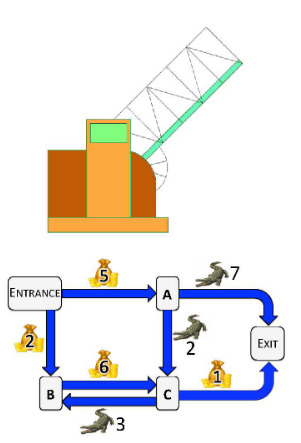
\includegraphics[width=0.40\textwidth]{images/mazy_luc_problem.png}\\[1.5cm]
}

\author
{
    \textbf{Realizado por:}\\[0.1cm] Pedro Grilo (43012) \\ Diogo Castanho (42496)\\[1cm]
}

\date{Ano Letivo 2020/2021}

% -------------------------------------------------------------------------------------------
%                                Body                                                       %
% -------------------------------------------------------------------------------------------

\begin{document}
\maketitle

% -------------------------------------------------------------------------------------------
\section{Introdução} 
\hspace{0,5cm}O Dirk vai enfrentar um novo desafio. O desafio consiste em andar num labirinto, com vários corredores ligados entre si, que fazem a conexão entre vários quartos existentes.

Na entrada, o Dirk recebe um cartão com um total de 0 créditos. Em cada corredor existe ou uma bolsa com moedas, ou uma ponte sobre um lago com crocodilos. Se o Dirk quiser passar esse corredor de crocodilos, terá de pagar um conjunto de moedas pedido para que a ponte seja baixa. 

Se ele não tiver moedas suficientes, terá que usar o seu cartão de crédito, podendo ficar com saldo negativo.\\
% -------------------------------------------------------------------------------------------
\section{Objetivos}

\hspace{0,5cm}Foi-nos proposta a realização de um trabalho que consistia na implementação de um programa que tem como objetivo receber um input onde nos é disponibilizado o número de quartos e o número de corredores do labirinto que o Dirk vai percorrer.

Também devem ter os corredores e pesos respetivos existentes (exemplo: Quarto1 para Quarto2, com 5 moedas, ou Quarto2 para Quarto4, com ponte de custo 3 moedas).

Com estes dados, devemos conseguir dizer se o Dirk ao chegar ao quarto final, perdeu ou não dinheiro.\\
% -------------------------------------------------------------------------------------------
\section{Descrição do Algoritmo}
\hspace{0,5cm}Após algumas interpretações falhadas na abordagem à resolução do problema, percebemos que o algoritmo mais adequado seria o algoritmo de \textbf{Bellman Ford}, uma vez que é um bom algoritmo para cálculo do caminho mais curto de um nó \textbf{Source} para os restantes nós do grafo.

Por sabermos que teríamos de pensar no problema como um grafo, criámos 2 classes: uma para os \textbf{Vértices} e outra para os \textbf{Arcos}.

Os vértices são constituídos por uma \textbf{Label}, que reprensenta o número dos mesmos, por um Vertice \textbf{Predecessor}, que irá conter o Vértice anterior a ele, e por uma \textbf{Distância}, que reprensenta a distância do caminho mais curto desde o vértice inicial até ele mesmo.

Os arcos são constituídos por dois vértices: um vértice \textbf{Source} e um vértice \textbf{Destination}. Para além disso tem um \textbf{peso}, que representa o custo de ir do vértice source para o vértice destination.

Na leitura do input fazemos logo a criação de todos os vértices (desde 0 até o valor do número de quartos - 1), colocando todos os vértices num array.

De seguida, mediante os seguintes inputs (dos arcos corredores, e do seu peso), críamos os arcos correspondentes a esses valores, colocando-os também num outro array.

Como no input temos duas letras: \textbf{B} para caminho com moedas, e \textbf{C} para caminho com ponte, tivemos que alterar o valor do peso para negativo quando fosse a letra C, facilitando a criação dos arcos com o peso correto.

De seguida chamamos a função \textbf{Bellman Ford}, onde o algoritmo vai ser efetuado, com os vértices e arcos gerados anteriormente.

Inicializamos um array auxiliar, que irá conter as distâncias de cada vértice até ao vértice inicial.
Para esse array damos logo à posição inicial o valor 0 (pois o vértice inicial tem distância 0).\\[0.5cm]

\large\textbf{CONTINUAÇÃO DA DESCRIÇÃO DO ALGORITMO}\\

Como feito na aula, tivemos que inicializar todos os valores dos vértices numa função \textbf{Initializa-Single-Source}, dando ao vértice source a distância 0. Aos outros vértices damos o valor de \textbf{+infinito}, dando ao atributo predecessor o valor \textbf{null}.

Após a atribuição correta dos valores aos vértices, passamos para a parte de \textbf{Relaxamento}, que podia ser numa função Relax à parte, mas decidimos fazê-la no código em si.

Nesta parte, vamos ter dois ciclos: o \textbf{exterior}, onde vamos de 1 até ao número de vértices existentes, e no ciclo \textbf{interior} vamos de 0 até ao número de arcos existentes.

Dentro deste ciclo, se o \textbf{valor da distância do vértice source do arco + o peso do grafo} for \textbf{menor que a distância do vetor destination do arco}, fazemos as \textbf{novas atribuições ao valor da distância do vértice destination desse arco, como também o seu vértice predecessor}.

Adicionamos também ao \textbf{array das distâncias do indíce do vértice destination}, o \textbf{alor da distância do vértice source + o valor do peso do arco} correspondente.

Para ver se existem ciclos negativos, fizemos mais outro for desde 0 até ao número de arcos, repetindo o if anterior, e para o caso de haver, retornar true pois quer dizer que encontra um deles.

Depois disto tudo, fizemos um \textbf{if} para ver se o \textbf{valor da distância do vértice final} até ao \textbf{vértice inicial}l era \textbf{negativa}, porque se fosse, o Dirk teria \textbf{perdido dinheiro}, retornando \textbf{true}.

Se nada destes ifs acontecesse, retornamos \textbf{false} pois quer dizer que o Dirk conseguiu fazer um caminho sem perda de dinheiro.\\
% -------------------------------------------------------------------------------------------
\section{Descrição dos Grafos}
\hspace{0,5cm}A partir do input inicial do primeiro exemplo, temos o seguinte grafo:\\
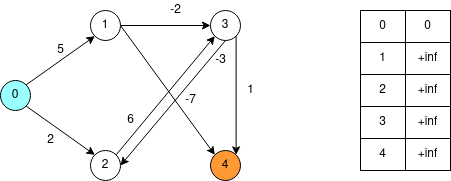
\includegraphics[width=0.5\textwidth]{images/grafo_inicial.png}

\textbf{Primeiro Relaxamento} - O \textbf{Vértice 0 irá "alargar"} para \textbf{os seus adjacentes 1 2}, onde estes passam a ter \textbf{distâncias 5 e 2} respetivamente.

\textbf{Segundo Relaxamento} - De seguida o \textbf{Vértice 1 irá alargar} dando ao vértice 3 o valor da  \textbf{distância 3} e ao vértice 4 a \textbf{distância -2}.

\textbf{Terceiro Relaxamento} - Posteriormente o \textbf{Vértice 2 irá alargar} não alterando o valor do seu vértice adjacente 3 (pois ficaria com distância superior à atual).

\textbf{Quarto Relaxamento} - O \textbf{Vértice 3 irá alargar} alterando o \textbf{valor de 4} que estava com \textbf{distância negativa}, passando a ter 3+1 = \textbf{4} de distância. Como o valor da distância do vértice 2 (adjacente de 3) estava em 2, este irá alterar o valor deste para 0 porque \textbf{5+(-2)+(-3) = 0 menor que 2}.\\[3cm]
\large\textbf{CONTINUAÇÃO DA DESCRIÇÃO DOS GRAFOS}\\[0.5cm]
Pelo que, as \textbf{distâncias finais} seriam:\\[0.5cm]
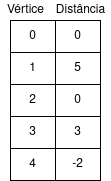
\includegraphics[width=0.2\textwidth]{images/quadro_dists_final.png}\\
% -------------------------------------------------------------------------------------------
\section{Análise de Complexidades}
\subsection{Complexidade Temporal}
\hspace{0,5cm}Para a complexidade temporal a função que irá ter \textbf{mais influência} sobre esta será a \textbf{função Bellman-Ford}.

Na função temos dois ciclos for: o ciclo exterior que vai de 1 até ao número de vértices (que representa o número de quartos do input). O ciclo interior vai de 0 até ao número de arcos disponíveis (que representa o número de corredores do input).\\[0cm]

Pelo que o \textbf{ciclo exterior} irá ter \textbf{complexidade de O(n)}, onde \textbf{n} representa o \textbf{número de vértices} do grafo, e o \textbf{ciclo interior} terá \textbf{complexidade de O(m)}, onde \textbf{m} representa o \textbf{número de arcos}.\\

Podemos então assim dizer que a \textbf{complexidade temporal do programa} será de \textbf{O(m * n)}.\\

\subsection{Complexidade Espacial}
\hspace{0,5cm}Assumindo a Complexidade Espacial de acessos a arrays e a métodos de classes (como get.source de um arco) tem sempre complexidade constante ( O(1)), não interferindo no resultado final desta.\\

Pelo que o que terá \textbf{importância} é:\\
O \textbf{array de vértices} com \textbf{tamanho n} (sendo n o número de vértices) tem \textbf{complexidade espacial O(n)}.
O \textbf{array de arcos} com \textbf{tamanho m} (sendo m o número de arcos) com \textbf{complexidade espacial O(m)}.
O \textbf{array das distâncias} com \textbf{\tamanho d} (sendo d o número de vértices novamente) com \textbf{complexidade espacial O(d)}.\\

Por isso, a \textbf{complexidade espacial} será \textbf{O(n * m * d)}.
% -------------------------------------------------------------------------------------------
\newpage
\section{Conclusão e Comentários Extra}
\hspace{0,5cm}Concluindo, o grupo teve algumas dificuldades iniciais na escolha do algoritmo, e posteriormente numa boa implementação do mesmo (problemas relacionados com os ciclos do algoritmo), tendo também problemas com a complexidade do mesmo, pois tinhamos métodos que para cada vértice que queríamos procurar, fazia um for para encontrar a sua label, o que aumentava significativamente a mesma (resolvido com a criação dos arrays para vértices e arcos, uma abordagem muito mais simples e eficaz).\\

Para além disso, o grupo ficou a entender muito melhor o algoritmo dado, tendo a certeza que o trabalho ajudará futuramente em próximas avaliações teóricas que o contenham.
% -------------------------------------------------------------------------------------------
\end{document}